% vim:spelllang=en_us:spell

\chapter{Introduction}

When developing software, one commonly relies on software libraries written by
other developers. To avoid introducing defects into the software, one has to
follow rules laid by the library developer. This includes the syntax of the
library and semantics of operations provided by the library. In a concurrent
environment, a new set of problems related to the proper synchronization of
threads is introduced.

\emph{Contracts for concurrency} enable library developers to define
restrictions on the usage of the library in a concurrent environment. In its
basic form, it specifies which method sequences must be executed atomically.
There are two extensions for contracts for concurrency. \emph{Parametric
contracts} allow one to better identify methods that need to be executed
atomically.  Contracts with \emph{spoilers} allow finer control over which
thread interleavings breach the contract. To verify that a program satisfies the
restrictions given by contracts for concurrency, one may use either static or
dynamic analysis, both offering different advantages.

The goal of this project is to design a dynamic analyzer that will be able to
detect contract violations in Java programs. To observe the behavior of the
program under analysis, the program must be modified to report all actions of
interest to the analyzer. That is usually done at the byte code level, and it
requires a lot of skill not to affect the behavior of the program under
analysis. Fortunately, the \emph{RoadRunner} framework takes care of the
instrumenting and provides a simple interface for observing actions taken by the
program under analysis. The contract analyzer will be built upon the RoadRunner
interface.

To successfully perform the analysis, the following must be done. A grammar for
contract definitions and a parser must be created. The instrumentation performed
by RoadRunner needs to be extended to extract additional information about the
program under analysis. Then finally, an analyzer for parametric contracts with
spoilers must be implemented using the RoadRunner interface. This master's
thesis deals with the design of the analyzer, its implementation, and the
evaluation of the analyzer.

The thesis is structured as follows. Chapter \ref{chTwo} describes specifics of
multi-threaded programming in Java, Java memory model, and an overview of
software errors related to concurrency. Approaches to the dynamic analysis of
Java programs and instrumentation techniques are described. Two important
frameworks are presented, the ASM framework for byte code instrumentation, and
the RoadRunner framework for writing dynamic analyzers. Chapter \ref{chThree}
introduces contracts for concurrency, their modified versions, and a method for
dynamic detection of contract violations. In Chapter \ref{chFour}, a dynamic
analyzer for contracts is designed. Chapter \ref{chFive} provides implementation
details and testing approaches.



\chapter{Dynamic Analysis of Multi-threaded Programs in Java}
\label{chTwo}

This chapter focuses on a dynamic analysis that detects errors related to
improper synchronization between threads in multi-threaded Java programs. In the
first section, dynamic analysis is compared with other approaches to software
verification. Then the most common types of errors found in multi-threaded
programs are presented. The following section explains the basics of
multi-threaded programming in Java. Then the most important concepts from the
Java memory model are described.

The second part of this chapter deals with the techniques used for dynamic
analysis of Java programs. The ASM framework for Java bytecode manipulation is
introduced along with brief overview of the Java virtual machine. Finally, the
RoadRunner framework is described in detail, as it is the basis for
implementation of the contract analyzer.


\section{Approaches to Software Verification}
\label{approachesToSwVerification}

The goal of software verification is to make sure that the software meets all
requirements. There are several approaches to software verification, each of
them having its own advantages and disadvantages. This section provides a
summary of testing, dynamic and static analysis, abstract interpretation,
theorem proving, and model checking.

\paragraph{Testing}
\emph{Testing} consists of running the software under different conditions and
checking the results of the computation (or observing other behavior of the
software). To gain enough confidence that the software operates correctly in all
conditions, a suitable set of \emph{test cases} must be found, which is
difficult, and sometimes impossible. Testing is best suited for confirming
the presence of defects in software, not for proving their absence
\cite{fundamentals}.

An important property of test cases is their \emph{repeatability}, meaning that
a certain test case will always yield the same result. When testing
multi-threaded programs, this property does not hold because of the
non-determinism introduced by the thread scheduler. Threads are interleaved
differently on each execution which means that errors may or may not appear.
This makes discovering defects in multi-threaded programs difficult.

\paragraph{Dynamic Analysis}
\emph{Dynamic analysis} works with information gathered during an execution of a
program. The information may be analyzed during program execution
(\emph{on-the-fly}) or at the end (\emph{post-mortem}). Even though the analysis
works with information from a single execution, it can in some cases find errors
that were not observed during the execution but may demonstrate themselves in
similar executions \cite{letko}. The dynamic analysis also suffers from
nondeterministic scheduling. The program under analysis may also behave
differently due to being observed by the analyzer.

The analyzer proposed in this thesis performs on-the-fly dynamic analysis of
contracts for concurrency and detects contract violations that occurred not only
in the given run but also those that may have occurred in similar runs.

\paragraph{Static Analysis}
\emph{Static analysis} is performed at compile-time and it does not require the
program to be running. The analysis is theoretically able to cover all possible
executions of a program. In practice, it is limited by the fact that the number
of thread interleavings in multi-threaded programs grows exponentially
\cite{letko}.

\paragraph{Abstract Interpretation}
\emph{Abstract interpretation} takes the source code and symbolically executes
it line by line, approximating the semantics of the program without performing
all the calculations. It suffers from similar problems as static analysis.

\paragraph{Model Checking}
\emph{Model checking} is a technique for checking whether a system satisfies
certain correctness specification \cite{letko}. It is based on systematic or
heuristic exploration of the state space. The drawback of this technique is that
the state space of the program model can be huge.

\paragraph{Theorem Proving}
\emph{Theorem proving} is a semi-automated approach to proving that a certain
facts are satisfied in the system. It is based on assumptions and general
theorems about the system and uses mathematical reasoning.


\section{Safety Errors in Multi-threaded Programs}

Contracts for concurrency specify rules on using a set of methods in a
concurrent setting. They aim at discovering errors specific to a concurrent
environment. When compared to single-threaded programs, multi-threaded programs
may encounter a whole new class of errors related to sharing memory between
threads. Errors presented in this section are classified as \emph{safety errors}
in \cite{letko} as these are usually checked in various dynamic analyses.

\paragraph{Data Race}
A \emph{data race} occurs when there are two unsynchronized accesses to a shared
variable and at least one of them is a write access.

\paragraph{Atomicity Violation}
When a code block is required to be atomic, all program executions must be
equivalent to an execution where the block is executed serially. Contract for
concurrency primarily focus on atomicity violations \cite{contracts}.

\paragraph{Order Violation}
When certain operations are required to be executed
in a certain order, and the order is not met in a given program execution, an
\emph{order violation} occurs. Contracts for concurrency can also detect order
violations \cite{contracts}.

\paragraph{Deadlock}
General definition of a deadlock is presented in
\cite{letko}. A program state contains a set $S$ of deadlocked threads if, and
only if each thread in $S$ is blocked and waiting for some event that could
unblock it, but such an event could only be generated by a thread from $S$.

\paragraph{Missed Signal}
A \emph{missed signal} is present in a program execution when one or more
threads are waiting for a signal, and the signal is never delivered.

\section{Multi-threaded Programming in Java}

Java provides built-in support for multi-threaded programming. This section
describes a typical thread life cycle, synchronization of threads, and
inter-thread communication, as these are important in dynamic analysis using
contracts.

A thread in Java is represented by a \texttt{Thread} object. There are two ways
to create a thread: by extending the \texttt{Thread} class, or by implementing
the \texttt{Runnable} interface. Both approaches produce a \texttt{Thread}
instance that executes the \texttt{run} method in a new thread when started.

To start a thread, the \texttt{start} method must be called (which will in
turn call the \texttt{run} method). The thread will terminate upon returning
from the \texttt{run} method. The \texttt{join} method is used in other
threads to wait for a thread to terminate \cite{javaTheCompleteReference}.
Figure \ref{threadExtend} shows a thread creation example by extending the
\texttt{Thread} class, Figure \ref{threadRunnable} shows the same example
achieved by implementing the \texttt{Runnable} interface.

\begin{figure}[hbt]
    \label{threadExtend}
\begin{lstlisting}[language=java]
class MyThread extends Thread {
  @Override
  public void run() {
    System.out.println("This is executed in a new thread.");
  }

  public static void main(String args[]) {
    MyThread t = new MyThread();
    t.start();
    t.join();
  }
}
\end{lstlisting}
    \caption{Creating a thread by extending the \texttt{Thread} class.}
\end{figure}

\begin{figure}[hbt]
    \label{threadRunnable}
\begin{lstlisting}[language=java]
class MyRunnable implements Runnable {
  public void run() {
    System.out.println("This is executed in a new thread.");
  }

  public static void main(String args[]) {
    Thread t = new Thread(new MyRunnable());
    t.start();
    t.join();
  }
}
\end{lstlisting}
    \caption{Creating a thread by implementing the \texttt{Runnable} interface.}
\end{figure}

When accessing a shared resource from multiple threads, proper synchronization
is usually required. In Java, every object gets an implicit monitor, which can
be owned by only one thread at a given time. To enter the monitor, one must use
either synchronized methods or synchronized statements.  \emph{Synchronized
statements} are code blocks with an explicitly specified object whose monitor is
entered before executing the block. \emph{Synchronized methods} enter the
monitor of the instance they are called upon. Figure \ref{synchronized} shows
examples of synchronized blocks and synchronized methods.

\begin{figure}[hbt]
    \label{synchronized}
\begin{lstlisting}[language=java]
class Example {
  private int a = 0;

  public synchronized void inc1() {
    a++;
  }

  public void inc2() {
    synchronized (this) {
      a++;
    }
  }
}
\end{lstlisting}
    \caption{The \texttt{inc1} method is \emph{synchronized}, on each call, the
    \texttt{Example} instance's monitor is entered. The \texttt{inc2} method is
    not synchronized but contains a \emph{synchronized block} with an explicitly
    specified monitor (\texttt{this}).}
\end{figure}

Communication between threads is achieved using the following methods:
\texttt{wait}, \texttt{notify}, and \texttt{notifyAll}. All methods must be
called within a synchronized context. Calling \texttt{wait} will suspend the
calling thread until some other thread enters the same monitor and calls either
\texttt{notify} or \texttt{notifyAll}.

Multi-threaded programs may use the \texttt{volatile} type modifier. It tells
the compiler that the variable may be modified outside of the current thread.
\todo{elaborate}

\section{Java Memory Model}

% http://www.cs.umd.edu/~pugh/java/memoryModel/jsr-133-faq.html
% https://docs.oracle.com/javase/specs/jls/se8/html/jls-17.html#jls-17.4.5

\emph{Java memory model} describes how threads in Java interact with each other
using shared memory. The model defines several relations that are used by the
dynamic analysis of contracts for concurrency, most notably the
\emph{happens-before} relation and the \emph{synchronizes-with} relation.

Java memory model takes a program and an execution trace, and for each read
operation decides if it is valid or not. The decision depends on the write
operation that modified the data before the read operation. The compiler,
runtime, and hardware must ensure that all executions of a program produce
execution traces that are valid according to the model \cite{jmmspec}.

In a single-threaded program, it is only required that the program produces the
same result as if it was run serially. The compiler is free to reorder
instructions when it does not affect the result of the computation.

In multi-threaded programs, the reordering of instructions has to be limited
when the threads interact with each other. In the model, only certain program
\emph{actions} are considered. There are several orders defined over the actions
which are used by the dynamic contract analysis: program order, synchronization
order, and happens-before order.

The actions can be either intra- or inter-thread. An \emph{inter-thread} action
can be detected or influenced by another thread. An \emph{intra-thread} action
is for example adding two local variables and it is not important to the model.
Non-volatile reading or writing of a shared variable is an inter-thread action.
\emph{Synchronization actions} are inter-thread actions that include volatile
reading or writing of variables, locking and unlocking of monitors, and starting
and stopping of a thread. Figure \ref{threadActions} shows examples of different
kinds of actions.

\begin{figure}[hbt]
    \label{threadActions}
\begin{lstlisting}[language=java]
class MySharedData {
  int mySharedVar = 0;

  public synchronized void MyMethod() {
    // synchronization action (entering a monitor)
    // intra-thread action (writing a local variable)
    int a = 42;
    // 2 inter-thread actions (reading and writing a shared variable)
    mySharedVar += a;
    // synchronization action (leaving a monitor)
  }
}
\end{lstlisting}
    \caption{Different program actions classified from the Java Memory Model
    point of view. Entering and leaving \texttt{MyMethod} produces
    \emph{synchronization actions}. Accessing \texttt{mySharedVar} is considered
    as an \emph{inter-thread} action, but not as a synchronization action
    because \texttt{mySharedVar} is not declared as \texttt{volatile}.}
\end{figure}


\emph{Program order} is a total order over all inter-thread actions from a given
thread. It reflects the order in which these actions would be executed if
run by the intra-thread semantics.

\emph{Synchronization order} is a total order over all synchronization actions
of an execution. Within each thread, the synchronization order is consistent
with the program order. The \emph{synchronized-with} relation is defined on
certain actions. For example: starting a thread is \emph{synchronized-with}
the first action in the new thread.

\emph{Happens-before order} is a partial order. If an action
\emph{happens-before} another, the first action is visible to and ordered before
the second action. If actions \emph{x} and \emph{y} belong to the same thread
and \emph{x} comes before \emph{y} in program order, then \emph{x happens-before
y}.  If \emph{x synchronizes-with y}, then \emph{x happens-before y}. Figures
\ref{hb1} and \ref{hb2} illustrates the \emph{happens-before} relation in simple
programs.

A \emph{data race} occurs, when there are two accesses to the same variable, at
least one of which is write, and these accesses are not ordered by
\emph{happens-before}. This situation is illustrated in Figure \ref{hb2}.

\begin{figure}[hbt]
    \label{hb1}
    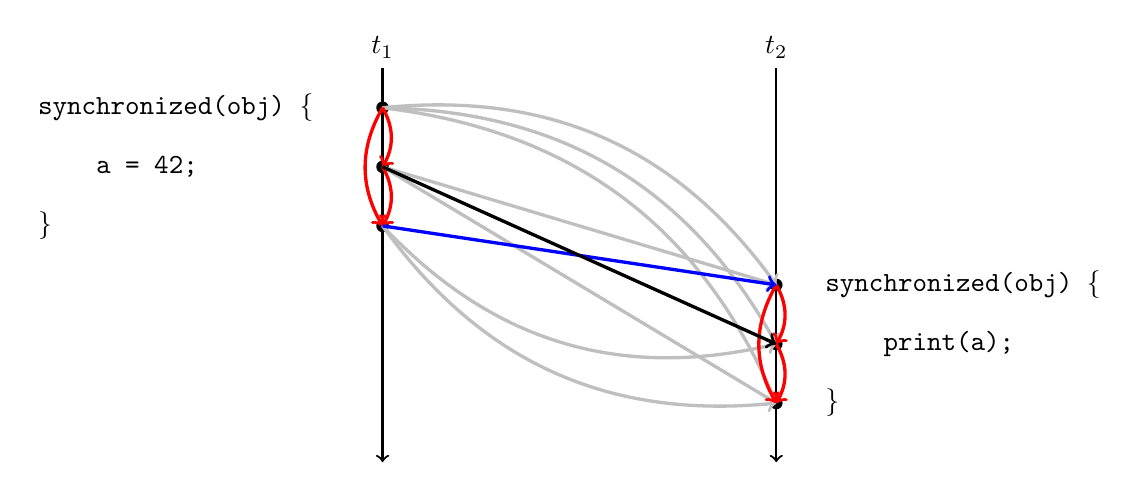
\begin{tikzpicture}
    \draw [->, thick] (4.5,0.5) node[above] {$t_1$} -- (4.5,-4.5);
    \draw (0,0) node[right] {\texttt{synchronized(obj) \{}};
    \coordinate (a1) at (4.5,0);
    \fill (a1) circle (0.08);
    \draw (0,-0.75) node[right] {\texttt{\quad \quad a = 42;}};
    \coordinate (a2) at (4.5,-0.75);
    \fill (a2) circle (0.08);
    \draw (0,-1.5) node[right] {\texttt{\}}};
    \coordinate (a3) at (4.5,-1.5);
    \fill (a3) circle (0.08);

    \draw [->, thick] (9.5,0.5) node[above] {$t_2$} -- (9.5,-4.5);
    \draw (10,-2.25) node[right] {\texttt{synchronized(obj) \{}};
    \coordinate (b1) at (9.5,-2.25);
    \fill (b1) circle (0.08);
    \draw (10,-3) node[right] {\texttt{\quad \quad print(a);}};
    \coordinate (b2) at (9.5,-3);
    \fill (b2) circle (0.08);
    \draw (10,-3.75) node[right] {\texttt{\}}};
    \coordinate (b3) at (9.5,-3.75);
    \fill (b3) circle (0.08);

    \draw[->,color=lightgray,very thick] (a1) to[bend left] (b1);
    \draw[->,color=lightgray,very thick] (a1) to[bend left] (b2);
    \draw[->,color=lightgray,very thick] (a1) to[bend left] (b3);
    \draw[->,color=lightgray,very thick] (a2) to (b1);
    \draw[->,color=lightgray,very thick] (a2) to (b3);
    \draw[->,color=lightgray,very thick] (a3) to[bend right] (b2);
    \draw[->,color=lightgray,very thick] (a3) to[bend right] (b3);

    \draw[->,color=red,very thick] (a1) to[bend left] (a2);
    \draw[->,color=red,very thick] (a2) to[bend left] (a3);
    \draw[->,color=red,very thick] (a1) to[bend right] (a3);

    \draw[->,color=red,very thick] (b1) to[bend left] (b2);
    \draw[->,color=red,very thick] (b2) to[bend left] (b3);
    \draw[->,color=red,very thick] (b1) to[bend right] (b3);

    \draw[->,color=blue,very thick] (a3) to (b1);

    \draw[->,very thick] (a2) to (b2);
\end{tikzpicture}

    \caption{\emph{Happens-before} relations in a correctly synchronized program
    consisting of threads $t_1$ and $t_2$. Each arrow represents a
    \emph{happens-before} relation. The red arrows represent the program order,
    the blue arrow represents the \emph{synchronizes-with} relation. Grey arrows
    complete the transitive closure. The conflicting accesses to variable
    \texttt{a} are not data races, because they are ordered by
    \emph{happens-before} (the black arrow).}
\end{figure}

\begin{figure}[hbt]
    \label{hb2}
    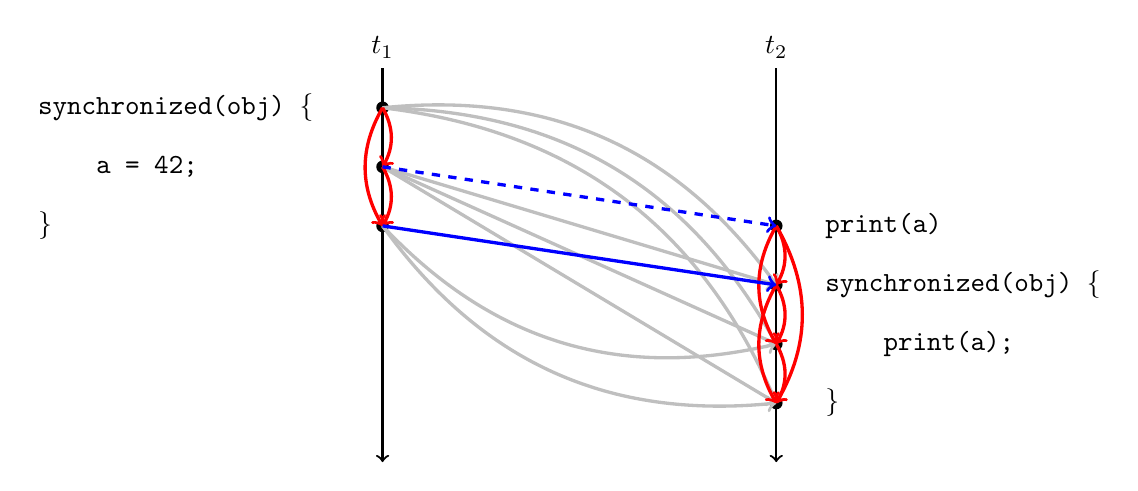
\begin{tikzpicture}
    \draw [->, thick] (4.5,0.5) node[above] {$t_1$} -- (4.5,-4.5);
    \draw (0,0) node[right] {\texttt{synchronized(obj) \{}};
    \coordinate (a1) at (4.5,0);
    \fill (a1) circle (0.08);
    \draw (0,-0.75) node[right] {\texttt{\quad \quad a = 42;}};
    \coordinate (a2) at (4.5,-0.75);
    \fill (a2) circle (0.08);
    \draw (0,-1.5) node[right] {\texttt{\}}};
    \coordinate (a3) at (4.5,-1.5);
    \fill (a3) circle (0.08);

    \draw [->, thick] (9.5,0.5) node[above] {$t_2$} -- (9.5,-4.5);
    \draw (10,-1.5) node[right] {\texttt{print(a)}};
    \coordinate (b0) at (9.5,-1.5);
    \fill (b0) circle (0.08);
    \draw (10,-2.25) node[right] {\texttt{synchronized(obj) \{}};
    \coordinate (b1) at (9.5,-2.25);
    \fill (b1) circle (0.08);
    \draw (10,-3) node[right] {\texttt{\quad \quad print(a);}};
    \coordinate (b2) at (9.5,-3);
    \fill (b2) circle (0.08);
    \draw (10,-3.75) node[right] {\texttt{\}}};
    \coordinate (b3) at (9.5,-3.75);
    \fill (b3) circle (0.08);

    \draw[->,color=lightgray,very thick] (a1) to[bend left] (b1);
    \draw[->,color=lightgray,very thick] (a1) to[bend left] (b2);
    \draw[->,color=lightgray,very thick] (a1) to[bend left] (b3);
    \draw[->,color=lightgray,very thick] (a2) to (b1);
    \draw[->,color=lightgray,very thick] (a2) to (b2);
    \draw[->,color=lightgray,very thick] (a2) to (b3);
    \draw[->,color=lightgray,very thick] (a3) to[bend right] (b2);
    \draw[->,color=lightgray,very thick] (a3) to[bend right] (b3);

    \draw[->,color=red,very thick] (a1) to[bend left] (a2);
    \draw[->,color=red,very thick] (a2) to[bend left] (a3);
    \draw[->,color=red,very thick] (a1) to[bend right] (a3);

    \draw[->,color=red,very thick] (b0) to[bend left] (b1);
    \draw[->,color=red,very thick] (b0) to[bend right] (b2);
    \draw[->,color=red,very thick] (b0) to[bend left] (b3);
    \draw[->,color=red,very thick] (b1) to[bend left] (b2);
    \draw[->,color=red,very thick] (b2) to[bend left] (b3);
    \draw[->,color=red,very thick] (b1) to[bend right] (b3);

    \draw[->,color=blue,dashed,very thick] (a2) to (b0);

    \draw[->,color=blue,very thick] (a3) to (b1);
\end{tikzpicture}

    \caption{\emph{Happens-before} relations in an incorrectly synchronized
    program (each solid arrow represents a \emph{happens-before} relation).
    There is no \emph{happens-before} relation between conflicting accesses
    \texttt{a=42} and \texttt{print(a)} (the dashed line), creating a data
    race.}
\end{figure}


\section{Instrumentation of Java Bytecode}

\emph{Instrumentation} is the act of inserting instructions into an existing
program to extract useful information at runtime. Instrumentation can be used to
measure performance, log events, or perform dynamic analysis. The running
program should not be aware that it is being instrumented and the result of the
computation should remain the same. Instrumentation may add significant overhead
to the program. For example, programs instrumented by the RoadRunner framework
are roughly 10 times slower \cite{RoadRunner}.

In Java, the instrumentation is done by changing the bytecode. There are several
general-purpose frameworks for modifying the Java bytecode. In this section, the
ASM framework is described as it is used by the RoadRunner framework, which is
the basis of this master's thesis.

\subsection{Java Bytecode Overview}

Programs written in Java are compiled into Java bytecode which is executed by
the Java Virtual Machine. Every class gets compiled into a Java class file
containing the following sections \cite{asmguide}:
\begin{itemize}
    \item Section with information about the class itself, such as the name of
    the class, the super class, implemented interfaces, and class annotations.
    \item One section per field, containing the field name, type, modifiers, and
    annotations.
    \item One section per method (and constructor), containing the name of the
    method, the return type, type of parameters, annotations, and compiled code
    of the method.
\end{itemize}

Java class files also contain a \emph{constant pool} section that holds all
numeric, type, and string constants which are then referenced from other
sections of the file. The whole structure is shown in Table \ref{classfile}.
The Java class file format is described in detail in the Java Virtual Machine
Specification \cite{jvmspec}.

\begin{table}
    \begin{center}
        \label{classfile}
        \begin{tabular}{|l|l|l|}
            \hline
            \multicolumn{2}{|l|}{Modifiers, name, super class, interfaces} \\
            \hline
            \multicolumn{2}{|l|}{Constant pool} \\
            \hline
            \multicolumn{2}{|l|}{Annotations} \\
            \hline
            \multicolumn{2}{|l|}{Attributes} \\
            \hline
            \multirow{3}{*}{Fields} & Modifiers, name, type \\
            & Annotations \\
            & Attributes \\
            \hline
            \multirow{3}{*}{Methods} & Modifiers, name, return and parameter types \\
            & Annotations \\
            & Attributes \\
            & Code \\
            \hline
        \end{tabular}
        \caption{Structure of the Java class file. Adapted from \cite{asmguide},
        simplified.}
    \end{center}
\end{table}

The Java Virtual Machine operates on two kinds of types: \emph{primitive types}
and \emph{reference types}. Examples of primitive types are \texttt{int},
\texttt{long}, \texttt{boolean}, or \texttt{double}. There are three kinds of
reference types: class types, array types, and interface types. The array type
consists of a component type which can also be an array type. For example,
\texttt{int[]} represents an array type with component type of \texttt{int}. All
reference types may hold a special null reference, which is also the default
value of reference types.

Compiled classes do not contain any \texttt{package} or \texttt{import}
statements, so all type names must be fully qualified. Internally, class files
use slashes instead of dots in type names, so for example
\texttt{java.lang.Object} becomes \texttt{java/lang/Object}. In most places,
Java types are represented with \emph{type descriptors}. Each primitive type is
assigned a single character: \texttt{I} for \texttt{int}, \texttt{D} for
\texttt{Double}, and so on. Classes and interfaces are written with prefix
\texttt{L} and semicolon at the end, so \texttt{String} becomes
\texttt{Ljava/lang/String;}. Arrays are represented using a
\texttt{\leftbracket} and the element type, so an array of integers is
\texttt{\leftbracket I}, an array of strings is \texttt{\leftbracket
Ljava/lang/String;}. Similarly, \emph{method descriptors} are used to represent
the return type of a method and types of all method parameters. For example, a
method declared as \texttt{double m(int i, String s)} would be represented as
\texttt{(ILjava/lang/String;)D}. In method descriptors, \texttt{V} is used when
the method returns \texttt{void}.

When executing, on each method invocation, the Java Virtual Machine creates a
new \emph{frame}. Each frame contains its own local variables and an operand
stack. When the method invocation is completed, the frame is destroyed.

Local variables are addressed by indexing. Each variable can hold a single value
of a primitive or reference type with the exception of \texttt{long} and
\texttt{double} which require a pair of variables. At index 0, there is a
reference to the object the method was invoked on (the value of \texttt{this} in
Java). Class methods (marked as \texttt{static} in Java) do not use this index.
Starting at index 1 (or 0 in case of class methods), method parameters are
stored. After the parameters, local variables may be stored.

Each frame contains an \emph{operand stack}, which is initially empty. Various
instructions are used to load values onto the stack, either from local variables
or fields. Other instructions take operands from the stack and push the result
back. When calling other methods, the parameters are also prepared on the stack.

Java Virtual Machine instructions can be divided into several categories. Load
and store instructions move values between local variables and the operand
stack. For example, the \texttt{iload\_3} instruction pushes the value (which is
of type \texttt{int}) from the local variable at index 3 to the operand stack.
Arithmetic instructions usually take two values from the operand stack, compute
the result, and store it back on the stack. For example, the \texttt{fmul}
instruction will multiply two values of type \texttt{float}. Type conversion
instructions convert the value on the top of the stack. Control transfer
instructions, such as \texttt{ifeq} or \texttt{goto}, cause the execution of
instruction other then the immediately following.

To create new arrays and objects, instructions \texttt{new}, \texttt{newarray},
and \texttt{anewarray} are used. Methods are invoked using these five
instructions: \texttt{invokevirtual}, \texttt{invokeinterface},
\texttt{invokespecial}, \texttt{invokestatic}, and \texttt{invokedynamic}, each
used in slightly different circumstances. Exceptions are thrown using the
\texttt{athrow} instruction. Entering a monitor is achieved by
\texttt{monitorenter} and \texttt{monitorexit} instructions, which are used by
synchronized statements in Java. An example of a method represented by bytecode
is shown in Figure \ref{bytecodeExample}.

\begin{figure}[hbt]
    \label{bytecodeExample}
    \begin{lstlisting}
public void foo(java.io.FileWriter, int, int)
  descriptor: (Ljava/io/FileWriter;II)V
  flags: (0x0001) ACC_PUBLIC
  Code:
    stack=2, locals=5, args_size=4
       0: iload_2
       1: iload_3
       2: iadd
       3: istore        4
       5: aload_1
       6: iload         4
       8: invokevirtual #2    // Method java/io/FileWriter.write:(I)V
      11: aload_1
      12: invokevirtual #3    // Method java/io/FileWriter.close:()V
      15: return
    \end{lstlisting}
    \caption{An example of a method bytecode viewed using the \texttt{javap}
    command. The method takes three parameters: a file writer and two integers.
    There are 5 local variables: the object the method was called on (index 0),
    method parameters (indices 1 to 3), and a local variable (index 5). On lines
    0 to 3, the two integers are loaded on to the operand stack, added together,
    and the result is stored in a local variable. Lines 5 to 7 calls the
    \texttt{write} method on the file writer, lines 11 and 12 calls the
    \texttt{close} method. Operands on lines 8 and 12 are indices to the
    constant pool section.}
\end{figure}


\subsection{The ASM framework}

The ASM framework allows generating and modifying Java classes directly in
bytecode. It can be used both statically (for example during compilation) or
dynamically (to create classes at runtime). The ASM framework provides an
interface for loading and storing the bytecode using higher-level abstractions,
such as constants, identifiers, methods, fields, etc. \cite{asmguide}.

There are two interfaces available: the \emph{core API} with an
\emph{event-based} representation of classes, and the \emph{tree API} with an
\emph{object-based} representation. The core API processes classes sequentially.
When parsing a class, the ASM parser will produce an event for each element of
the class.  When writing a class, the writer creates the class based on a
sequence of events. The tree API loads the whole class and creates a tree of
objects representing the class. The core API is faster and requires less memory,
however, it is not practical for complex transformations \cite{asmguide}. The
RoadRunner framework uses the core API.

The core API is based on the \texttt{ClassVisitor} abstract class. The class
contains methods for visiting different sections of a class, for example,
\texttt{visitAttribute}, \texttt{visitMethod}, or \texttt{visitField}. Complex
sections, such as methods or fields, have their visitor classes. For example,
the \texttt{MethodVisitor} class contains methods such as
\texttt{visitLocalVariable}, \texttt{visitCode}, or \texttt{visitParameter}
\cite{asmguide}.

To generate a new class, one has to create a \texttt{ClassWriter} instance,
which is a subclass of \texttt{ClassVisitor}. Then a sequence of visit methods
must be called, such as \texttt{visitField} or \texttt{visitMethod}. The
\texttt{ClassWriter} instance will generate appropriate bytecode on each call.

To read and parse a class, one has to create a \texttt{ClassReader} instance.
The reader will produce a sequence of events for each section of the class. To
consume those events, a \texttt{ClassVisitor} instance must be given to the
reader. The reader will then call appropriate visit methods on the visitor as it
is parsing the class. To demonstrate this, one can create a \texttt{ClassReader}
and connect it to a \texttt{ClassWriter} (which is a subclass of
\texttt{ClassVisitor}). The reader will call visit methods on the writer,
effectively copying the class.

\begin{figure}[hbt]
    \label{asmArchitecture}
    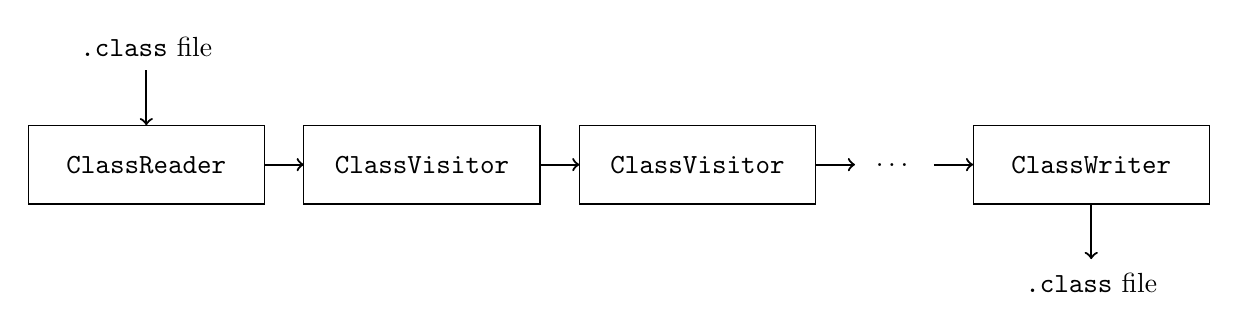
\begin{tikzpicture}
    \draw (0,1.5) node {\texttt{.class} file};
    \draw [->, thick] (0,1.2) -- (0,0.5);
    \draw (-1.5,0.5) rectangle (1.5,-0.5);
    \draw (0,0) node {\texttt{ClassReader}};
    \draw [->, thick] (1.5,0) -- (2,0);
    \draw (2,0.5) rectangle (5,-0.5);
    \draw (3.5,0) node {\texttt{ClassVisitor}};
    \draw [->, thick] (5,0) -- (5.5,0);
    \draw (5.5,0.5) rectangle (8.5,-0.5);
    \draw (7,0) node {\texttt{ClassVisitor}};
    \draw [->, thick] (8.5,0) -- (9,0);
    \draw (9.5,0) node {\ldots};
    \draw [->, thick] (10,0) -- (10.5,0);
    \draw (10.5,0.5) rectangle (13.5,-0.5);
    \draw (12,0) node {\texttt{ClassWriter}};
    \draw [->, thick] (12,-0.5) -- (12,-1.2);
    \draw (12,-1.5) node {\texttt{.class} file};
\end{tikzpicture}

    \caption{Typical architecture for class transformation.}
\end{figure}

The typical class transformation uses the following architecture (see Figure
\ref{asmArchitecture}): a \texttt{ClassReader} instance reads the class, then
one or more \texttt{ClassVisitor} instances modify the class, and then a
\texttt{ClassWriter} instance writes the modified class back to a file.

\section{Dynamic Analysis using RoadRunner}
\label{roadRunnerUsage}

The RoadRunner framework is used for the dynamic analysis of concurrent programs
written in Java. RoadRunner instruments programs to obtain a stream of events
that are useful for dynamic analysis, such as memory accesses, synchronizing on
a lock, forking or joining of threads, and so on. This event stream is then
available to various analysis tools. Multiple tools can be chained together,
each tool acting as a filter over the events. This allows complex analyses to be
built from simpler, modular tools \cite{RoadRunner}.

RoadRunner aims to simplify writing dynamic analysis tools. A RoadRunner
analysis tool only needs to handle events of interest. RoadRunner will ensure
that the event is properly detected and the event handler is called. To store
the state of the analysis, RoadRunner provides support for associating data with
memory locations, locks, or threads.

\todo{tool composition}
\todo{optional: debugging, comparing analyses}

\subsection{The RoadRunner Programming Interface}

Every analyzer in RoadRunner is based on the \texttt{Tool} class. Figure
\ref{toolclass} contains the most important methods of \texttt{Tool}. During the
analysis, every time an action is detected, the appropriate method in
\texttt{Tool} is called, along with an \texttt{Event} object that contains
information about the event.

\begin{figure}[hbt]
    \label{toolclass}
    \begin{lstlisting}[language=java]
public abstract class Tool {
  // event handlers for accessing a memory location
  public void access(AccessEvent fae) { }
  public void volatileAccess(VolatileAccessEvent fae) { }
  // event handlers for entering and exiting methods
  public void enter(MethodEvent me) { }
  public void exit(MethodEvent me) { }
  // event handlers for locking
  public void acquire(AcquireEvent ae) { }
  public void release(ReleaseEvent re) { }
  // event handlers for thread events
  public void preJoin(JoinEvent je) { }
  public void postJoin(JoinEvent je) { }
  public void preStart(StartEvent se) { }
  public void postStart(StartEvent se) { }
  // shadow location initialization
  public ShadowVar makeShadowVar(AccessEvent ae) { }
}
    \end{lstlisting}
    \caption{The abstract class \texttt{Tool}. Only selected public methods are
    shown.}
\end{figure}

The following events are detected by the RoadRunner framework:
\begin{itemize}
    \item Method entry and exit.
    \item Memory accesses -- reads and writes to fields and variables.
    \item Lock acquires and releases.
    \item Synchronization signals -- wait and notify.
    \item Thread forking and joining.
\end{itemize}

There are several subclasses of the \texttt{Event} class with specific
information about events.

RoadRunner allows associating data with objects from the program under analysis.
For each thread, a \texttt{ShadowThread} object is created which contains a
reference to the underlying thread. Similarly, for each lock, a
\texttt{ShadowLock} object is created. Both extend the \texttt{Decoratable}
class that allows storing of arbitrary information. For associating data with
memory locations, a \emph{shadow location} is created when the location is first
accessed.

Multiple tools can be chained together. Each event handler method forwards the
\texttt{Event} instance to the next tool in the chain by default. If the event
is not forwarded, the tool becomes a filter over the event stream. This can be
used to filter out events that are not interesting to a particular analysis and
then performing the analysis in the next tool.

\subsection{RoadRunner Synchronization Models}

In RoadRunner, all threads of the program under analysis generate events. The
events are also handled by the same thread that generated them which means that
several event handlers may be running concurrently. Tools written for RoadRunner
must provide internal synchronization to ensure that no concurrency-related
errors occur in the tool itself. RoadRunner contains an option to serialize all
events. In this mode, there is only one event handler running at a time.

\subsection{Instrumentation Performed by RoadRunner}

RoadRunner uses a modified version of the ASM framework to instrument the
program under analysis. Before a class is loaded, it is instrumented. The
instrumented code will then produce events that will be sent to the tool chain
for an analysis. Three important kinds of actions are instrumented: field
accesses, method invocations, and monitor entries and exits.

Field accesses are instrumented by adding two new methods for each field: one
for reading and one for writing to the field. In these methods, write and read
events are generated. In the rest of the code, all \texttt{getfield} and
\texttt{putfield} instructions are replaced with calls to the corresponding
access methods. RoadRunner allows tools to store arbitrary data related to a
field in \emph{shadow variables}. For each field, a new field of the
\texttt{ShadowVar} type is created to store the data. Figures \ref{rrInstBefore}
and \ref{rrInstField} shows a simple class before and after field
instrumentation.

\begin{figure}[hbt]
    \label{rrInstBefore}
    \begin{lstlisting}
private int bar;

public void foo();
   0: aload_0
   1: aload_0
   2: getfield      #2    // Field bar:I
   5: bipush        42
   7: iadd
   8: putfield      #2    // Field bar:I
  11: return\end{lstlisting}
    \caption{An example class bytecode viewed using the \texttt{javap} tool,
    simplified.}
\end{figure}

\begin{figure}[hbt]
    \label{rrInstField}
    \begin{lstlisting}
public int bar;

public transient rr.state.ShadowVar __(*\$*)rr_bar;

public void __(*\$*)rr_put_bar(int, int, rr.state.ShadowThread)
  (code omitted)

public int __(*\$*)rr_get_bar(int, rr.state.ShadowThread)
  (code omitted)

public void foo();
   0: invokestatic  #51 // Method rr/state/ShadowThread
                        // .getCurrentShadowThread:()Lrr/state/ShadowThread;
   3: astore_2
   4: aload_0
   5: aload_0
   6: iconst_1
   7: aload_2
   8: invokespecial #56 // Method __$rr_get_bar:(ILrr/state/ShadowThread;)I
  11: bipush        42
  13: iadd
  14: iconst_2
  15: aload_2
  16: invokespecial #53 // Method __$rr_put_bar:(IILrr/state/ShadowThread;)V
  19: return\end{lstlisting}
    \caption{Code from Figure \ref{rrInstBefore} instrumented by RoadRunner. For
    the \texttt{bar} field, two access methods are added and a new field of type
    \texttt{ShadowVar}. In the \texttt{foo} method, the \texttt{bar} field is
    accessed using methods \texttt{\_\_\$rr\_get\_bar} and
    \texttt{\_\_\$rr\_put\_bar}. These methods take the current shadow thread as
    an argument which is obtained by calling \texttt{getCurrentShadowThread}.}
\end{figure}

Method invocations are tracked by creating a wrapper method for each method. The
original method is renamed, but otherwise left intact (the code may however be
further instrumented to obtain other information, such as field accesses). Then
a wrapper method with the same name as the original one is created. The wrapper
method generates enter and exit events. In order to detect abnormal method exits
that are caused by an exception being thrown, the call to the original method is
wrapped in a try block. When an exception is caught, the exit event is generated
and the exception is re-thrown. An example of a method instrumented by
RoadRunner is shown in Figure \ref{rrInstMethod}.

\begin{figure}[hbt]
    \label{rrInstMethod}
    \begin{lstlisting}
public int __(*\$*)rr_foo__(*\$*)rr__Original_(int);
   0: invokestatic  #20 // Method rr/state/ShadowThread
                        // .getCurrentShadowThread:()Lrr/state/ShadowThread;
   3: astore_3
   4: iload_1
   5: ireturn

public int foo(int);
   0: invokestatic  #20 // Method rr/state/ShadowThread
                        // .getCurrentShadowThread:()Lrr/state/ShadowThread;
   3: astore_3
   4: aload_0
   5: sipush        508
   8: aload_3
   9: invokestatic  #27 // Method rr/tool/RREventGenerator
                        // .enter:(Ljava/lang/Object;ILrr/state/ShadowThread;)V
  12: aload_0
  13: iload_1
  14: invokespecial #29 // Method __(*\$*)rr_foo__(*\$*)rr__Original_:(I)I
  17: aload_3
  18: invokestatic  #33 // Method rr/tool/RREventGenerator
                        // .exit:(Lrr/state/ShadowThread;)V
  21: goto          29
  24: aload_3
  25: invokestatic  #33 // Method rr/tool/RREventGenerator
                        // .exit:(Lrr/state/ShadowThread;)V
  28: athrow
  29: ireturn\end{lstlisting}
    \caption{Method \texttt{int foo(int a)} instrumented by RoadRunner. The
    original method was renamed to \texttt{\_\_\$rr\_foo\_\_\$rr\_\_Original\_}
    and a new method with the original name was created. This method generates
    enter and exit events and calls the original method.}
\end{figure}

Monitor entries and exits are handled differently for synchronized statements
and synchronized methods. Synchronized statements in Java are represented by
\texttt{monitorenter} and \texttt{monitorexit} instructions. RoadRunner extends 
all occurrences of these instructions with calls to methods that generate
acquire and release events. Synchronized methods in Java do not need
\texttt{monitorenter} and \texttt{monitorexit} instructions, the locking is
performed implicitly by the Java Virtual Machine. In RoadRunner, synchronized
methods are replaced with synchronized statements that are then instrumented as
described above. For each synchronized method, a wrapper method is created. The
original method's synchronized flag is cleared. The wrapper method, which is
also not synchronized, contains a synchronized statement with call to the
original method. Synchronized methods are in the end wrapped twice, the first
wrapper generates synchronization events and the second one generates method
invocation events.

\chapter{Contracts for Concurrency}
\label{chThree}

When developing software, one frequently uses modules created by someone else
via its programming interface. For example, in object-oriented programming, the
interface consists of public methods of a given class. Accessing the interface
requires one to follow a protocol consisting of: (i) syntax, i.e. types of
parameters and return values, (ii) semantics, i.e. the expected behavior for
given input parameters, and (iii) access restrictions. Access restrictions
include the domain of valid values, dependencies on other services, and
atomicity violations \cite{contracts}.

\emph{Contracts for concurrency} \cite{FITPUB10817},
\cite{DBLP:journals/corr/SousaDFL15}, are a case of a software protocol that
expresses access restrictions in a concurrent setting. In its basic form, they
specify sequences of methods that must be executed atomically. The contracts can
be extended with parameters to reflect the data flow between the methods (so
that only methods manipulating the same data must be executed atomically).
Another extension adds so-called \emph{spoilers} (so that given sequence must be
executed atomically only with respect to only certain sequences). Both
extensions can be combined. This chapter defines basic contracts, as well as
both extensions to them. Then a method for dynamic validation of contracts for
concurrency is presented. The analyzer, implemented in this thesis, is based on
this method.

\section{Basic Contracts}
\label{basicContracts}

A \emph{contract} is formally defined in \cite{FITPUB10817} as follows. Let
$\Sigma_\mathbb{M}$ be a set of all public method names (the API) of a module or
a library. A \emph{contract} is a set $\mathbb{R}$ of \emph{clauses}. Each
clause $\varrho \in \mathbb{R}$ is a regular expression over
$\Sigma_\mathbb{M}$. A contract violation occurs when any of the sequences in a
contract is interleaved with an execution of a method from $\Sigma_\mathbb{M}$
over the same object.

\emph{Example.} Consider a map implementation with the following operations:
\texttt{put(key, value)}, \texttt{get(key)}, \texttt{remove(key)}, and
\texttt{contains(key)}. Then a contract for this class may contain the following
clauses:
\begin{align*}
    (\varrho_1) &\ \texttt{put get}\\
    (\varrho_2) &\ \texttt{contains (put|get|remove)}
\end{align*}
Clause $\varrho_1$ states that when an element is put into the map and then
retrieved, it should be executed atomically (because the element may be removed
between the calls). Clause $\varrho_2$ states that when the program modifies the
map based on the result of the \texttt{contains} call, it should be atomic.

\section{Parametric Contracts}
\label{parametricContracts}

In some situations, the definition of contracts may be too restrictive,
producing false alarms. In \cite{contracts}, contracts are extended with
parameters to reflect the data flow between methods. Consider the following
example:
\begin{lstlisting}[language=java]
if (q.contains(42)) q.remove(42);
\end{lstlisting}

These two calls must be executed atomically only if they share the same
argument. This dependency can be expressed using \emph{meta-variables} placed as
the parameters or return values of methods. Parameters that should not be taken
into account are marked with free meta-variable (denoted with an underscore).

\emph{Example.} The example from section \ref{basicContracts} can be extended
with parameters:
\begin{align*}
    (\varrho_1) &\ \texttt{put(X,\_) \_ = get(X)}\\
    (\varrho_2) &\ \texttt{\_ = contains(X) ( put(X,\_) | \_ = get(X) |
    remove(X) )}
\end{align*}

The basic definition of contracts contains one implicit parameter, the object
that the method was called upon (\texttt{this} in Java) \cite{FITPUB10817}. To
better illustrate this, the example can be rewritten as:
\begin{align*}
    (\varrho_1) &\ \texttt{X.put(Y,\_) \_ = X.get(Y)}\\
    (\varrho_2) &\ \texttt{\_ = X.contains(Y) ( X.put(Y,\_) | \_ = X.get(Y) |
    X.remove(Y) )}
\end{align*}


\section{Contracts with Spoilers}
\label{contractsWithSpoilers}

In \cite{contracts}, contracts are extended with contextual information to
distinguish which method sequences violate the contract. Each clause of the
basic contract is called a \emph{target} and is assigned a set of so-called
\emph{spoilers}. A spoiler is a set of method sequences that may violate its
target.

Consider clause $\varrho_1$ from the example in Section \ref{basicContracts}. If
the element that was put into the map is concurrently removed or updated before
the \texttt{get} call, a contract violation should be detected.  However,
calling \texttt{contains} or \texttt{get} on the element will not affect the
computation and should not be marked as a contract violation. In this example,
methods \texttt{put} and \texttt{remove} are spoilers for a target
$\varrho_1$, denoted as \texttt{put get} $\leftsquigarrow$ \texttt{put|remove}.

% TODO: this is basically copied - is it ok?

Formally, as defined in \cite{contracts}, let $\mathbb{R}$ be the set of
\emph{target} clauses where each target $\varrho \in \mathbb{R}$ is a regular
expression over $\Sigma_\mathbb{M}$. Let $\mathbb{S}$ be the set of
\emph{spoilers} where each spoiler $\sigma \in \mathbb{S}$ is a regular
expression over $\Sigma_\mathbb{M}$. A \emph{contract} is a relation $\mathbb{C}
\subseteq \mathbb{R} \times \mathbb{S}$ defining for each target, which spoilers
may cause atomicity violation.

Contract violation is observed when a target sequence $\varrho \in \mathbb{R}$
is fully interleaved by a spoiler sequence $\sigma \in \mathbb{C}(\varrho)$ and
the sequences are executed on the same object.

\emph{Example.} The example from section \ref{basicContracts} can be extended
with spoilers:
\begin{align*}
    (\varrho_1) &\ \texttt{put get} \leftsquigarrow \texttt{put|remove}\\
    (\varrho_2) &\ \texttt{contains (put|get|remove)} \leftsquigarrow
    \texttt{put|remove}
\end{align*}

When combining parametric contracts with spoilers, the spoilers may also contain
parameters. Then a contract violation is detected only when spoiler arguments
match target arguments.

\emph{Example.} Examples from sections \ref{parametricContracts} and
\ref{contractsWithSpoilers} combined together:
\begin{align*}
    (\varrho_1) &\ \texttt{X.put(Y,\_) \_ = X.get(Y)} \leftsquigarrow
    \texttt{X.put(Y,\_)|X.remove(Y)}\\
    (\varrho_2) &\ \texttt{\_ = X.contains(Y) ( X.put(Y,\_) | \_ = X.get(Y) |
    X.remove(Y) )}\\
    &\quad \leftsquigarrow \texttt{X.put(Y,\_)|X.remove(Y)}
\end{align*}


\section{Dynamic Contract Validation}

In \cite{contracts}, a dynamic contract validation method is proposed for
contracts with spoilers. Parametric contracts are not included in the method.
This section provides an overview of the method.

\subsection{Multi-threaded Program Traces}

In the context of the dynamic on-the-fly contract validation, multi-threaded
\emph{program trace} consists of events of the following types:
\begin{itemize}
    \item thread forking or joining another thread,
    \item thread entering or exiting a method,
    \item thread acquiring or releasing a lock.
\end{itemize}

All events in a trace are indexed by their position in the trace. Let
$\mathbb{T}$ be a set of threads, $\mathbb{R}$ a set of targets, $\mathbb{S}$ a
set of spoilers, $\mathbb{C} \subseteq \mathbb{R} \times \mathbb{S}$ a set of
contracts, and $\mathbb{L}$ a set of locks. The set of all events that can be
generated by a thread $t \in \mathbb{T}$ is then denoted as $\mathbb{E}_t$. Let
$\mathbb{E} = \bigcup_{t \in \mathbb{T}} \mathbb{E}_t$. A \emph{trace} is then a
sequence $\tau = e_1 \hdots e_n \in \mathbb{E}^+$.

% TODO: basically copied

Given a trace $\tau = e_1 \hdots e_n \in \mathbb{E}^+$, we call its subsequence
$r = e_{i_1} e_{i_2} \hdots e_{i_k}$, $1 < k \leq n$, an \emph{instance} of a
target $\varrho \in \mathbb{R}$ if, and only if:
\begin{enumerate}
    \item $r$ consists of well-paired method enter and exit events,
    \item all enter events of $r$ match the regular expression of $\varrho$,
    \item apart from events $e_{i_1},\ldots,e_{i_k}$, there is no event from the
        alphabet of $\varrho$ executed by $t$ between events $e_{i_1}$ and
        $e_{i_k}$.
\end{enumerate}

\emph{Example.} Given target $\varrho = abc$, and a trace $\tau_1 = adbdc$,
there is a target instance $r = e_1 e_3 e_4$. In trace $\tau_2 = acbdc$, there
is no target instance.

A \emph{spoiler instance} $s$ of a spoiler $\sigma \in \mathbb{S}$ is defined
similarly. We let $start(r) = e_{i_1}$ and $end(r) = e_{i_k}$ denote the first
and last events of a target, respectively. Likewise, $start(s)$ and $end(s)$
denote the first and last events of a spoiler, respectively.

\subsection{Contract Violation}

A contract is violated when there is a target instance that is fully interleaved
with a spoiler instance from another thread. The interleaving is defined using a
\emph{happens-before} relation, which is in the context of contracts defined as
follows \cite{contracts}. A \emph{happens-before relation} $\prec_{hb}$ over a
trace $\tau = e_1 \ldots e_n \in \mathbb{E}^+$ is the smallest transitively
closed relation on the set of events from $\tau$ such that $e_j \prec_{hb} e_k$
holds when $j < k$ and one of the following holds:
\begin{enumerate}
    \item both $e_j$ and $e_k$ are executed by the same thread,
    \item both $e_j$ and $e_k$ acquire or release the same lock,
    \item one of $e_j$ and $e_k$ is a fork or a join performed by thread $t$,
        and the other is executed by thread $u$.
\end{enumerate}

A contract $(\varrho,\sigma) \in \mathbb{C}$ is \emph{violated} in a trace
$\tau$ if, and only if there is a target instance $r$ in the trace and a spoiler
instance $s$ in the trace such that:
\begin{align*}
    start(s) \nprec_{hb} start(r) \wedge end(r) \nprec_{hb} end(s)
\end{align*}
The violation occurs when the spoiler may have started after the target started
and it may have ended before the target ended. When given a complete program
execution trace, all target and spoiler instances can be detected, the
happens-before relation can be deduced, and all contracts can be easily checked
for violations. The trace, however, can get large and make this approach
unpractical. For this reason, several optimizations are introduced in
\cite{contracts}, which are presented in the next section. An example of a
program trace containing a contract violation is shown in Figure \ref{traces}.

\begin{figure}[hbt]
    \begin{center}
        \label{traces}
        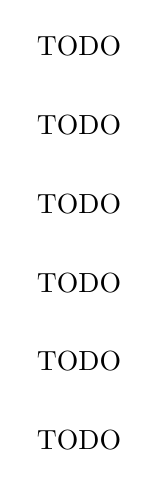
\begin{tikzpicture}
    \node at (0,0) (n1) {TODO};
    \node at (0,1) (n1) {TODO};
    \node at (0,2) (n1) {TODO};
    \node at (0,3) (n1) {TODO};
    \node at (0,4) (n1) {TODO};
    \node at (0,5) (n1) {TODO};
\end{tikzpicture}

        \caption{\todo{}}
    \end{center}
\end{figure}

\subsection{Vector Clocks}

\cite{fasttrack}

\todo{definition, usage, examples}
{\color{blue}\lipsum[1-3]}

\subsection{On-the-fly Contract Validation}

To check contract validations, it is not required to keep the entire program
execution trace. A \emph{trace window} is kept instead. Events are moved to the
trace window as soon as they become available and are removed under certain
conditions. The goal is to keep the window as small as possible.

Spoiler instances can be safely removed from the window whenever a contract
violation that would be detected with the spoiler can be detected without it. A
spoiler instance can be removed from the window whenever a newer instance of the
same spoiler is detected \cite{contracts}.

A target instance $r$ can be safely removed with respect to a spoiler instance
$s$ whenever a contract violation that would be detected between $r$ and $s$,
can be detected between $s$ and another target instance too. Note that target
instances may be removed only with respect to a given spoiler, not in general
\cite{contracts}.

To further reduce the required information about the trace, \emph{vector clocks}
are used. For each target and spoiler instance in the trace window, only vector
clocks of their beginning and end need to be kept.

The method for on-the-fly contract validation does the following. At method
entry events, target and spoiler sequences are detected. At method exit events,
it is detected whether a target or a spoiler instance has ended. When a target
instance ends, spoiler instances from the trace window are checked if they
violate the target. When a spoiler instance ends, target instances from the
trace window are checked if they are violated by the spoiler. At method exit,
target and spoiler instances are also discarded when no longer needed.

\section{Previous Work}

\todo{m. janousek, anaconda, results}
{\color{blue}\lipsum[1-2]}



\chapter{Design of a Dynamic Analyzer for Parametric Contracts with Spoilers}
\label{chFour}

This chapter describes the proposed dynamic analyzer for parametric contracts
with spoilers. The analyzer follows the method for dynamic analysis of contracts
described in \cite{contracts} and extends it to support parametric contracts.

The analyzer is built as a new tool for the RoadRunner framework. The input is a
program under analysis and a contract definition. The analyzer is then able to
detect contract violations in the program and report them. The RoadRunner
framework was modified to support obtaining method arguments and return values.

Section \ref{overview} provides an architectural overview of the analyzer
itself. Section \ref{constraining} describes several restrictions that were
placed on the analyzer in the design phase. In Section \ref{instrChanges},
necessary changes to RoadRunner itself are presented. Section \ref{contracts}
describes how a contract is defined and processed before the analysis is
started. The core function of the analyzer is described in Section
\ref{contractAnalyzer}. Section \ref{contractTool} describes how the analyzer
interacts with RoadRunner.

\section{Overview of the Contract Analyzer}
\label{overview}

This section provides a high-level overview of the contract analyzer. The
\texttt{ContractAnalyzer} class is the core of the analyzer. It receives events
from the program under analysis, detects target and spoiler instances, and looks
for contract violations. It manages data stored with threads and locks, such as
trace windows and vector clocks. The \texttt{ContractAnalyzer} class can be
instantiated without any dependencies from the RoadRunner project, which is
useful for testing purposes. A detailed description of \texttt{ContractAnalyzer}
can be found in Section \ref{contractAnalyzer}.

The \texttt{ContractTool} class is a subclass of RoadRunner's \texttt{Tool}
class. During the initialization of \texttt{ContractTool}, the contract
definition file is parsed and \texttt{ContractAnalyzer} is created. In
\texttt{ContractTool}, relevant methods are overridden to receive events from
RoadRunner, such as lock acquire and release or method exit. These events are
then processed and sent to \texttt{ContractAnalyzer}. Section \ref{contractTool}
provides a detailed description of \texttt{ContractTool} and Section
\ref{contracts} describes the parsing and representation of contracts.

For each thread, a \texttt{Window} instance is created by
\texttt{ContractAnalyzer}. It stores information about target and spoiler
instances in a trace window. On method exit, existing instances are advanced,
new instances are started, and for all finished instances, contract violations
are checked.

\section{Constraining Analyzer Capabilities}
\label{constraining}

The analyzer is designed with several restrictions based on the previous work,
such as \cite{janousek} or \cite{FITPUB10817}, to improve its performance.
First, a restriction is placed on the parameters in contract definitions to
reduce the number of instances in a trace window. Then the conditions for
removing instances from the trace window are discussed and a related contract
restriction is introduced. Finally, it is described how nested method calls
should be handled.

\subsection{Avoiding Cloning of Target and Spoiler Instances}

The method for analyzing contracts described in \cite{janousek} produces an
enormous number of instances being tracked at the same time. A lot of instances
are created because of the necessity to clone target and spoiler instances
before they are advanced. Consider the following target: \texttt{a(X) b(Y)
c(X,Y)} and the following program trace: \texttt{a(1) b(2) b(3) c(1,3)}.  When
\texttt{a(1)} enters the trace window, a new instance is created and the value
of \texttt{X} is set to 1. But when processing \texttt{b(2)}, the analyzer
cannot reliably decide whether the method call belongs to the instance or not
(there might be \texttt{c(1,2)} later in the trace). The only option is to keep
the instance and create a duplicate which is then advanced (while setting
\texttt{Y} to 2).

To prevent duplication of instances, the following restriction was put on the
contract definition. All target and spoiler parameters must be assigned in the
first call of a given target or spoiler. This ensures that there is no ambiguity
in deciding whether a given method call advances an instance or not. For
example, the target from the previous example is invalid because the value of
\texttt{Y} remains unknown after the first method call.

\subsection{Invalidating Instances}

A target or spoiler instance, as defined in Chapter \ref{chThree}, requires that
no method belonging to the alphabet of a given target or spoiler may be called
between the events that form the instance. In practice, it means that a running
instance must be discarded when a method belonging to the target or spoiler is
called. For example, consider a target \texttt{abc} and the following program
trace: \texttt{aa}. After the first \texttt{a}, a new instance is created. After
accepting the second \texttt{a}, the instance must be discarded.

When tracking parametric contracts, instances cannot be easily discarded.
Consider a running instance of a target (or a spoiler), all of its parameters
are assigned a value. When a method is called that belongs to the alphabet of
the instance's target, three kinds of situations can happen:
\begin{enumerate}
    \item The method matches the target definition and method arguments match
        the values of instance parameters. The instance is advanced with the
        method.
    \item The method matches the target definition but method arguments conflict
        with the values assigned to the instance. The instance cannot be
        advanced but it also should not be discarded. The method call most
        likely belongs to another instance.
    \item The method does not match the target definition. According to the
        definition in Chapter \ref{chThree}, the instance should be discarded.
        But the analyzer does not know if the method call is in any way related
        to the instance.
\end{enumerate}

The second situation can be illustrated in the following example. Consider a
target \texttt{a(X) b(X)} and a program trace \texttt{a(1) b(2) b(1)}. After
\texttt{a(1)}, an instance is created with \texttt{X} set to 1. When
\texttt{b(2)} is called, the value of \texttt{X} conflicts with the value
stored in the instance. However, the instance should not be discarded as we can
see that a matching call exists later in the trace.

An example of the third situation. Consider target \texttt{a(X) b(X)} and a
program trace \texttt{a(1) a(2) b(1) b(2)}. Intuitively, there should be two
instances detected, one with \texttt{X} set to 1, and one with \texttt{X} set to
2. After \texttt{a(1)}, the first instance with \texttt{X=1} is created. When
\texttt{a(2)} is accepted, the instance cannot be discarded even though it
belongs to the alphabet of the target.

The problems described above mean that the analyzer will never discard an
already running instance, the only option is to advance it. Another option is to
modify the behavior in the third situation so that the analyzer will try to
guess whether a method call belongs to the current instance or not. With simple
contracts, the decision can be easy. Consider the target from the previous
paragraph: \texttt{a(X) b(X)}. In this case, every time a method \texttt{b()} is
called, the analyzer can decide whether it belongs to the currently tracked
instance or not based on the value of \texttt{X}. The decision is less clear
when a target contains the same method multiple times with different parameters.
For example, consider target \texttt{a(X,Y) b(X) b(Y)} and a program trace
containing two interleaved instances with different parameters: \texttt{a(1,2)
a(2,3) b(2) b(1) b(2) b(3)}. After \texttt{a(1,2)}, a new instance is created
with \texttt{X=1} and \texttt{Y=2}. After \texttt{a(2,3)}, another instance is
created with \texttt{X=2} and \texttt{Y=3}. When \texttt{b(2)} is encountered,
the second instance is advanced, because it matches the target. The analyzer may
however discard the first instance because \texttt{b(2)} is contained in the
target as \texttt{b(Y)}, but the expected method was \texttt{b(X)}. It is not
clear, what the proper behavior should be. The analyzer should therefore never
discard running instances.

\subsection{Kleene Star in Contract Definition}

The analyzer never invalidates a running instance. This fact allows for
optimization in contract definitions. As defined in Chapter \ref{chThree}, a
target or a spoiler is a regular expression over methods. The analyzer should
therefore recognize contracts defined using all three basic operations:
concatenation (\texttt{ab}), alternation (\texttt{a|b}), and Kleene star
(\texttt{a*}). Due to the fact, that no method call can invalidate a running
instance, the Kleene star operation is not needed. All parts of an expression
that are also operands of a Kleene star operation can be removed with no impact
on the analysis. For example, a regular expression \texttt{ab*c} can be replaced
with \texttt{ac}. Calls to method \texttt{b} will be simply ignored. These
simplified regular expressions, when converted to a finite automaton, do not
create any loops. This allows for simpler structures in the implementation of
the analyzer.

\subsection{Nested Method Calls}

The method described in \cite{contracts} is based on program traces where
every method represents a single event in the trace. However, the RoadRunner
framework produces two events for every method -- method entry and method exit.
For parametric contracts, we need to obtain values of parameters and also the
return value, which is available only on method exit. For convenience, the
analyzer should use only the method exit event. This means that the analyzer may
produce unexpected results when the program under analysis contains nested calls
to methods that are part of the contract. Consider the following methods that
are both parts of a contract:

\begin{lstlisting}[language=java]
public void a() { b(); }
public void b() { ... }
\end{lstlisting}

After calling method \texttt{a()}, the trace recorded by the analyzer will be
\texttt{b() a()} instead of more intuitive \texttt{a() b()}.

\section{Changes to Instrumentation Performed by RoadRunner}
\label{instrChanges}

The RoadRunner framework does not expose the method arguments or the return
value through its API. For the tracking of parametric contracts, it is necessary
to obtain method arguments and return values so that the contract parameters
can be assigned values.

The \texttt{enter} and \texttt{exit} of RoadRunner's \texttt{Tool} class methods
both take a \texttt{MethodEvent} parameter containing the following information:
\begin{itemize}
    \item Target -- \texttt{null} for static methods, the value of \texttt{this}
        for instance methods.
    \item A \texttt{MethodInfo} object -- static information about the method
        definition (name, descriptor, whether it is synchronized or static).
    \item Call site location -- where was the method invoked.
\end{itemize}

The \texttt{MethodEvent} class was extended for storing method arguments and the
return value. The following methods were added:

\begin{lstlisting}[language=java]
public Object[] getArgs();
public void setArgs(Object[] args);
public Object getReturnValue();
public void setReturnValue(Object returnValue);
\end{lstlisting}

Arguments and return values which are reference values (class instances or
arrays) can be stored directly in the \texttt{Object} data type. Primitive
values (such as \texttt{int} or \texttt{float}) cannot be stored in
\texttt{Object} directly, they must be wrapped in a class instance. Each
primitive type has a corresponding object wrapper class, for example,
\texttt{int} is wrapped in the \texttt{java.lang.Integer} class. The
\texttt{getArgs()} method should return an array of size 0 for a method that
takes no arguments and it should return \texttt{null} when the arguments are not
available, for example when the argument instrumentation is turned off. The
\texttt{getReturnValue()} should return \texttt{null} when the value is not
available (for example on method entry), when the method throws an exception, or
when the method returns \texttt{void}.

\subsection{Parameter Matching}
When trying to advance a running instance, method arguments must be checked, if
they match the previously assigned parameters. For reference types, the equality
operator (\texttt{==}) is used which compares the addresses of both objects. For
primitive values that are wrapped in an object, the \texttt{equals()} method
must be used. As a result, the analyzer will always compare instances of wrapper
classes (such as \texttt{Integer}) by calling the \texttt{equals()} method, even
if the instance was created by the program under analysis. This may or may not
be the intended behavior and the user of the analyzer should be aware of this.

\section{Contracts Definition and Parsing}
\label{contracts}

Before the start of the analysis, a contract must be specified. This section
describes the syntax of a contract configuration file, how it is parsed, and how
it is represented in the analyzer.

\subsection{Contract Definition Syntax}

The analyzer takes a contract definition as a parameter. At the top level, the
definition contains pairs of targets and spoilers. Each target and spoiler is
represented by a regular expression over methods. The on-the-fly dynamic
analysis described in Chapter \ref{chThree} expects several spoilers to be
assigned to a single target. In practice, the spoilers can be merged into a
single regular expression so that each target has exactly one spoiler. Each
method is parametrized, including arguments, return value, and the object it is
called upon (\texttt{this}).

To specify methods unambiguously, method names must be fully qualified (for
example \texttt{java/lang/Object.toString}). Java allows method overloading, so
to distinguish methods with the same name but different number and type of their
parameters, the contract definition contains the method descriptor (for example
\texttt{(Ljava/lang/Object;)V}. Each method in a contract definition consists of
the enclosing class, the method name, the method descriptor, and a list of
meta-variables. For example:

\begin{lstlisting}
test/sanity/ArrayList.set(ILjava/lang/Object;)Ljava/lang/Object; X=Y(Z,_)
\end{lstlisting}

This represents the \texttt{set} method called on an \texttt{ArrayList} from
the \texttt{test.sanity} package. The first meta-variable \texttt{X} is the
return value, \texttt{Y} is the \texttt{ArrayList} instance, and \texttt{Z} is
the first parameter (integer). The second parameter (object) is marked with free
meta-variable (\texttt{\_}) meaning that the analyzer will ignore its value. The
return value or the target of the method can be omitted.

Targets and spoilers are defined using a limited regular expression over
methods. Concatenation is achieved simply by writing two methods, one after
another, alternation is denoted by a vertical bar (\texttt{|}). The Kleene star
operator (\texttt{*}) is not allowed. An example of a target definition:

\begin{lstlisting}
Test.a()V X() ( Test.b()V X() | Test.c()V X() )
\end{lstlisting}

A contract clause is defined as two regular expressions over methods, separated
by an arrow and a semicolon at the end. A contract is then a list of clauses. An
example of a full contract is shown in Figure \ref{contract}. The full grammar
for contracts is shown in Appendix \ref{appGrammar}.

\begin{figure}[hbt]
    \label{contract}
    \begin{lstlisting}
Map.put(ID)V M(K,_) Map.get(I)D M(K)
    <- Map.put(ID)V M(K,_) | Map.remove(I)D M(K) ;

Map.contains(I)Z M(K)
  ( Map.put(ID)V M(K,_) | Map.get(I)D M.(K) | Map.remove(I)D M(K) )
  <- Map.put(ID)V M(K,_) | Map.remove(I)D M(K) ;
\end{lstlisting}
    \caption{Contract from Chapter \ref{chThree} written for a Map with
    \texttt{int} keys and \texttt{double} values. The first target matches an
    inserting element to the map at a given key and then retrieving it. The
    target can be invalidated by calling either \texttt{put} or \texttt{get}
    with the same key. The second target matches checking if a key is present in
    the map and then modifying the value at the given key. The target can be
    invalidated by replacing the value or by removing it.}
\end{figure}

\subsection{Contract Representation}
All parts of a contract definition are parsed into a corresponding class
instance. Each method in a target or spoiler is represented by a
\texttt{Signature} instance. It consists of a method name, a fully qualified
name of the enclosing class, and a method descriptor. The method descriptor
contains information about parameter types. The main purpose of this class is to
be compared with method invocation events to determine if the invoked method
matches the method from a contract. Meta-variables are parsed into a
\texttt{MetaVars} instance.

Each target and spoiler is represented by a \texttt{State} instance that will
later be used to construct a finite automaton for detecting running target and
spoiler instances. A target with a single method will be represented by two
states: one starting state with a transition to an accepting state. The
transition will contain the method signature and meta-variables. During parsing
of more complex targets and spoilers, these one-method state structures are
combined. See Figure \ref{states} for an example. During the analysis,
\texttt{State} instances will be used for checking whether a given method
invocation can advance a given target or spoiler.

\begin{figure}[hbt]
    \begin{center}
        \label{states}
        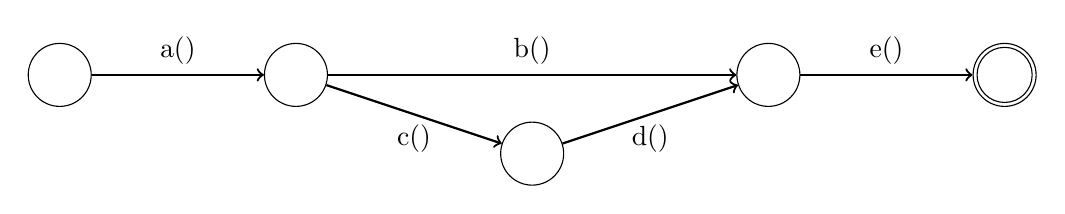
\begin{tikzpicture}[
    mystyle/.style={circle, minimum size=8mm, fill=white, draw=black}
]
    \node[mystyle] at (0,0) (n1) {};
    \node[mystyle] at (3,0) (n2) {};
    \node[mystyle] at (6,-1) (n3) {};
    \node[mystyle] at (9,0) (n4) {};
    \node[mystyle] at (12,0) (n5) {};

    \draw[->, thick] (n1) -- node[above] {a()} (n2);
    \draw[->, thick] (n2) -- node[above] {b()} (n4);
    \draw[->, thick] (n4) -- node[above] {e()} (n5);
    \draw[->, thick] (n2) -- node[below] {c()} (n3);
    \draw[->, thick] (n3) -- node[below] {d()} (n4);
    \draw[] (n5) circle (3.5mm);
\end{tikzpicture}

        \caption{A structure of states representing the following regular
        expression: \texttt{a(b|cd)e}.}
    \end{center}
\end{figure}

A contract is then made up of target--spoiler pairs. When a contract is created,
a set of all method signatures used in the contract is extracted. During the
analysis, the set of signatures is used to filter method invocations so that
only relevant methods are processed by the analyzer.

\section{Contract Analyzer}
\label{contractAnalyzer}
The main class, \texttt{ContractAnalyzer} receives events from the program under
analysis, detects target and spoiler instances in all threads, and looks for
contract violations when a target or spoiler instance finishes. The
\texttt{ContractAnalyzer} class provides the following interface:
\begin{itemize}
    \item A constructor that takes a \texttt{Contract} instance.
    \item \texttt{exit} method that is called on method exit. It takes a thread
        identifier, a method signature, and method arguments (also containing
        the return value). When a contract violation is detected, the
        \texttt{exit} method will throw an exception.
    \item \texttt{acquire} and \texttt{release} methods that are called when a
        synchronized block or a synchronized method is entered and exited. The
        methods both take a thread identifier and a lock identifier.
    \item \texttt{create} method that is called when a new thread is created. It
        takes a thread identifier.
    \item \texttt{fork} and \texttt{join} methods that take two thread
        identifiers.
\end{itemize}

The \texttt{ContractAnalyzer} class manages data stored with threads and locks.
When created by calling \texttt{create}, each thread will get a trace window and
a vector clock. Methods \texttt{acquire}, \texttt{release}, \texttt{fork}, and
\texttt{join} only modify vector clocks of threads and locks.

The \texttt{exit} method calls the trace window associated with a given thread.
The trace window receives method signature and arguments so that it can try to
advance all of its target and spoiler instances. It also receives the current
vector clock and references to trace windows of other threads so that it can
look for contract violations.

The \texttt{ContractAnalyzer} class is created and called by the
\texttt{ContractTool} class which directly uses the RoadRunner API. The
\texttt{ContractTool} class is described in Section \ref{contractTool}.

The interface of the analyzer is made up of synchronized methods to ensure
proper synchronization. This approach is not the same as the event serialization
mentioned in Chapter \ref{chTwo}. All events that are not calling analyzer's
methods will still be concurrent.

\subsection{Tracking of Target and Spoiler Instances}

For each thread, a \texttt{Window} object is kept during the analysis. It
contains target and spoiler instances present in a trace window. When a method
invocation is detected in a thread, all target and spoiler instances are
advanced (if possible) and new instances are started.

An instance is bound to a target or spoiler from the contract definition. The
instance is created by encountering the first method signature in a target or
spoiler. The instance is advanced to the next state and waits for the next
method as defined in the given target or spoiler. During the first transition,
values of all parameters are assigned. There can be multiple instances of the
same target or spoiler that vary only by the value of their parameters. Each
instance remembers the vector clock of its beginning.

When an instance is advanced using the last method in the target or spoiler
definition, it reaches an accepting state. At this point, the analyzer checks
for contract violations (see Section \ref{violations}). Then the instance is
reset. That means that the instance again waits for the first method signature
in a given target or spoiler. The value of parameters will however stay
unchanged. The vector clocks of the beginning and the end of the instance are
saved. So when an instance is running for the second time, it has access to the
vector clocks of a previously encountered instance. See Figure
\ref{instanceLifeCycle} for illustration of an instance life cycle.

\begin{figure}[hbt]
    \begin{center}
        \label{instanceLifeCycle}
        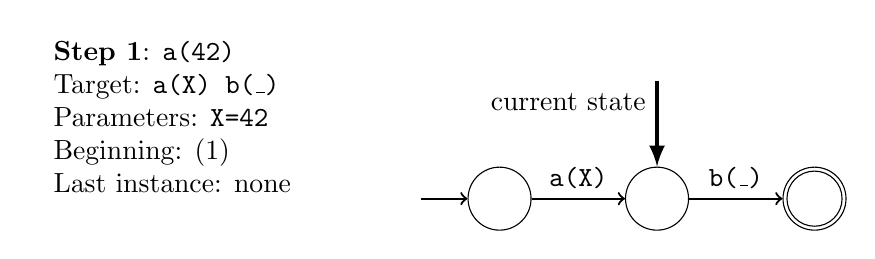
\begin{tikzpicture}[
    mystyle/.style={circle, minimum size=8mm, fill=white, draw=black}
]
    \node[mystyle] at (0,0) (n1) {};
    \node[mystyle] at (2,0) (n2) {};
    \node[mystyle] at (4,0) (n3) {};

    \draw[->, thick] (-1,0) -- (n1);
    \draw[->, thick] (n1) -- node[above] {\texttt{a(X)}} (n2);
    \draw[->, thick] (n2) -- node[above] {\texttt{b(\_)}} (n3);
    \draw[] (n3) circle (3.5mm);

    \draw[-latex, ultra thick] (2,1.5) -- node[near start, left] {current state} (n2);

    \node[anchor=west] at (-6,1) {\begin{tabular}{l}
        \textbf{Step 1}: \texttt{a(42)} \\
        Target: \texttt{a(X) b(\_)} \\
        Parameters: \texttt{X=42} \\
        Beginning: (1) \\
        Last instance: none
    \end{tabular}};
\end{tikzpicture}

        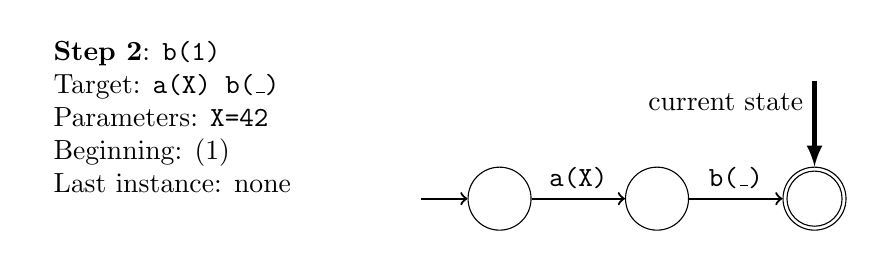
\begin{tikzpicture}[
    mystyle/.style={circle, minimum size=8mm, fill=white, draw=black}
]
    \node[mystyle] at (0,0) (n1) {};
    \node[mystyle] at (2,0) (n2) {};
    \node[mystyle] at (4,0) (n3) {};

    \draw[->, thick] (-1,0) -- (n1);
    \draw[->, thick] (n1) -- node[above] {\texttt{a(X)}} (n2);
    \draw[->, thick] (n2) -- node[above] {\texttt{b(\_)}} (n3);
    \draw[] (n3) circle (3.5mm);

    \draw[-latex, ultra thick] (4,1.5) -- node[near start, left] {current state} (n3);

    \node[anchor=west] at (-6,1) {\begin{tabular}{l}
        \textbf{Step 2}: \texttt{b(1)} \\
        Target: \texttt{a(X) b(\_)} \\
        Parameters: \texttt{X=42} \\
        Beginning: (1) \\
        Last instance: none
    \end{tabular}};
\end{tikzpicture}

        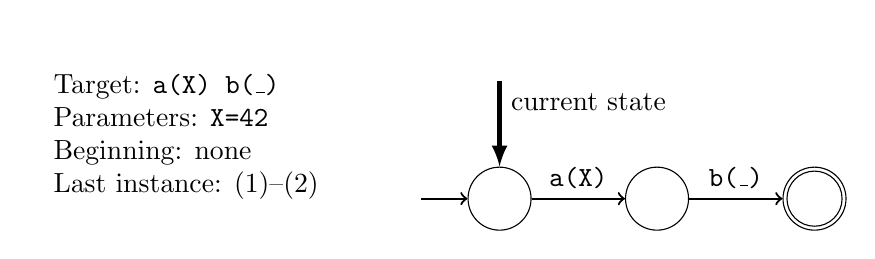
\begin{tikzpicture}[
    mystyle/.style={circle, minimum size=8mm, fill=white, draw=black}
]
    \node[mystyle] at (0,0) (n1) {};
    \node[mystyle] at (2,0) (n2) {};
    \node[mystyle] at (4,0) (n3) {};

    \draw[->, thick] (-1,0) -- (n1);
    \draw[->, thick] (n1) -- node[above] {\texttt{a(X)}} (n2);
    \draw[->, thick] (n2) -- node[above] {\texttt{b(\_)}} (n3);
    \draw[] (n3) circle (3.5mm);

    \draw[-latex, ultra thick] (0,1.5) -- node[near start, right] {current state} (n1);

    \node[anchor=west] at (-6,1) {\begin{tabular}{l}
        \\
        Target: \texttt{a(X) b(\_)} \\
        Parameters: \texttt{X=42} \\
        Beginning: none \\
        Last instance: (1)--(2)
    \end{tabular}};
\end{tikzpicture}

        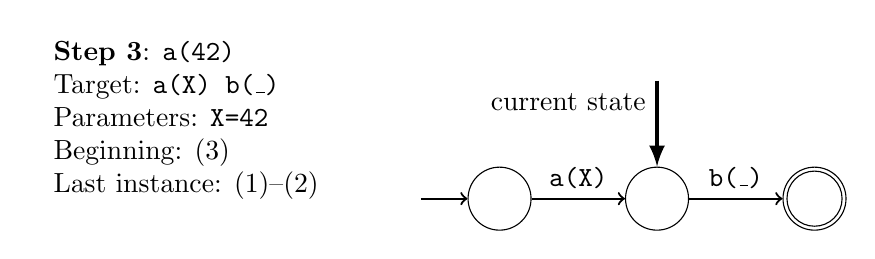
\begin{tikzpicture}[
    mystyle/.style={circle, minimum size=8mm, fill=white, draw=black}
]
    \node[mystyle] at (0,0) (n1) {};
    \node[mystyle] at (2,0) (n2) {};
    \node[mystyle] at (4,0) (n3) {};

    \draw[->, thick] (-1,0) -- (n1);
    \draw[->, thick] (n1) -- node[above] {\texttt{a(X)}} (n2);
    \draw[->, thick] (n2) -- node[above] {\texttt{b(\_)}} (n3);
    \draw[] (n3) circle (3.5mm);

    \draw[-latex, ultra thick] (2,1.5) -- node[near start, left] {current state} (n2);

    \node[anchor=west] at (-6,1) {\begin{tabular}{l}
        \textbf{Step 3}: \texttt{a(42)} \\
        Target: \texttt{a(X) b(\_)} \\
        Parameters: \texttt{X=42} \\
        Beginning: (3) \\
        Last instance: (1)--(2)
    \end{tabular}};
\end{tikzpicture}

        \caption{An example of an instance life cycle. In the first step, the
        instance is created when a method call \texttt{a(42)} is encountered.
        The vector clock of the beginning is set and the parameters are assigned
        a value. In step 2, the instance is fully accepted. At this point, the
        analyzer looks for contract violations. Then the instance is reset, the
        vector clock of the beginning is reset, and the vector clocks of the
        last instance are set. In step 3, method \texttt(a) is called with an
        argument that matches the value of \texttt{X} in the instance. The
        instance is started again.}
    \end{center}
\end{figure}

When a method call enters the trace window, all running instances (those with
parameters already assigned) are advanced. The method call may however also
start a new instance that is not yet part of the trace window. The analyzer
tries to create new instances from targets and spoilers from the contract. These
new instances are added to the trace window only if there is no matching
instance already present in the trace window. Two instances are matching, if
they are bound to the same target or spoiler, their parameters share the same
values, and they both just started (they accepted the same first method). In
practice, the only difference between these matching instances is that one
contains information about the previously encountered instance while the other
does not.

\emph{Example.} Consider target \texttt{a(X) b(X)} and a program trace
\texttt{a(1) b(1) a(2) b(2) a(1)}. After \texttt{a(1)}, the analyzer adds a new
instance $i_1$ to the window with \texttt{X=1}. After \texttt{b(1)}, $i_1$ is
advanced, accepted, and reset. No new instance is started because there is no
target starting with method \texttt{b}. After \texttt{a(2)}, $i_1$ cannot be
advanced, because the parameters do not match. New instance $i_2$ with
\texttt{X=2} is added to the trace window. After \texttt{b(2)}, $i_2$ is
advanced, accepted, and reset.  When \texttt{a(1)} is encountered again, $i_1$
is advanced but no new instance is added because $i_1$ would match the newly
created instance.

\subsection{Detection of Contract Violations}
\label{violations}

Each time a target or a spoiler is fully recognized by the analyzer, it must be
checked whether there are any contract violations. When a method enters a trace
window, there may be several instances from the same thread that will be fully
accepted by this method call. For each accepted target and spoiler instance, the
analyzer will look for conflicting instances in trace windows from other
threads.

When an instance is fully accepted, the analyzer will retrieve all
\emph{conflicting instances} from other threads. If the instance is a target
instance, the analyzer will retrieve instances of a spoiler that can invalidate
the target, as specified in the contract. Similarly, if the instance is a
spoiler instance, the analyzer will look for instances of a target that can be
invalidated by the spoiler. For each conflicting instance, it is checked whether
the contract parameter values match. Then finally, the analyzer checks the
vector clocks of each matching instance and decides if the two instances
interleave each other.

The two instances may not actually interleave each other. The interleaving is
decided based on the vector clocks of the beginnings and ends of the two
instances. Vector clocks are only updated when threads synchronize themselves.
So the analyzer will mark the two instances as interleaving when there was not
a synchronization between the threads that would prevent them to interleave each
other in another run of the program under analysis.

\todo{example}

\section{A Contract Analyzer Tool}
\label{contractTool}

The \texttt{ContractAnalyzer} class described in Section \ref{contractAnalyzer}
is not meant to be called directly by RoadRunner because it contains only
methods specific to the validation of contracts. The \texttt{ContractTool} class
was created as a layer between RoadRunner and \texttt{ContractAnalyzer}. Its
purpose is to load a contract from a file, create a \texttt{ContractAnalyzer}
instance, and forward relevant events from RoadRunner to
\texttt{ContractAnalyzer}.

The \texttt{ContractTool} class is a subclass of the \texttt{Tool} class (see
Section \ref{roadRunnerUsage}). The following methods are overridden:
\begin{itemize}
    \item \texttt{init}, which is called before the analysis, after
        command-line options are processed;
    \item \texttt{exit}, which is called when a method exits;
    \item \texttt{create}, which is called when a new thread is created;
    \item \texttt{acquire} and \texttt{release()}, which is called when a
        synchronized method or a synchronized block is entered or exited;
    \item \texttt{preStart}, which is called before a new thread is started
        (after a fork operation);
    \item \texttt{postJoin}, which is called after a thread is joined with
        another thread.
\end{itemize}

Methods for detecting memory accesses will not be used by the tool, and also no
data will be stored in shadow memory locations, except for vector clocks stored
with locks.

In its \texttt{init} method, the tool loads a contract definition from a file
and calls the contract parser. After the contract is parsed, it constructs
\texttt{ContractAnalyzer}.

The \texttt{exit} method extracts relevant data from \texttt{MethodEvent} that
is supplied by RoadRunner. Then it checks if the method exists in the contract,
and if it does, \texttt{ContractAnalyzer} is called. The method filtering
happens in \texttt{ContractTool} and not in \texttt{ContractAnalyzer} because it
is not essential to the analysis and also, there are several filtering solutions
available. In this master's thesis, the filtering is done by comparing method
signatures during the analysis. A better approach, which might be implemented in
the future, is to instrument only methods contained in a contract. In that case,
no filtering during analysis is needed as it is guaranteed that each method
event produced will belong to a method in the contract.

The rest of the methods, \texttt{create}, \texttt{acquire}, \texttt{release},
\texttt{preStart}, and \texttt{postJoin}, just pick relevant information from
events provided by RoadRunner and forward it to \texttt{ContractAnalyzer}.



\chapter{Implementation and Testing}
\label{chFive}

The analyzer described in Chapter \ref{chFour} was successfully implemented.
This chapter provides implementation details and clarifies decisions made during
the implementation. Section \ref{approaches} describes approaches and principles
that shaped the implementation. Before the implementation took place, several
RoadRunner dependencies were upgraded, see Section \ref{asmAndJava}. In Section
\ref{cfParsing}, the contract file parser is described. Changes to the
instrumentation performed by RoadRunner are described in detail in Section
\ref{instrImpl}. Finally, Section \ref{testing} describes testing approaches.

\section{General Approaches}
\label{approaches}
The implementation of the analyzer was guided by several principles or
approaches that are described in this section.

\subsection{Functional Programming}
The analyzer implementation uses several concepts from functional programming
which are briefly described in this section.

\paragraph{Immutable data structures}
All classes except for \texttt{ContractAnalyzer} and \texttt{ContractTool} are
immutable. Once created, the internal state of objects does not change. All
operations produce a new object instead of modifying the current one. See the
next section for more details.

\paragraph{Side effects and pure functions}
Most methods in the analyzer are pure functions, which means that each call can
be always replaced with a resulting value of the call. For example, consider
pure function \texttt{int sum(int a, int b)}. Then the method call
\texttt{sum(2,3)} can be always replaced with \texttt{5} without changing
program behavior. Pure functions perform no side effects (such as writing to a
file).

\paragraph{Higher-order function}
The analyzer contains and uses methods that take functions as parameters.

\subsection{Immutable Data Structures}

The data structures used by the analyzer are \emph{immutable}. An immutable
object is an object whose internal state remains constant after it has been
created.  This property brings several benefits. The object can be shared among
multiple threads without the need for synchronization. Immutable objects are
always in a consistent state. The public methods of a given class will always
behave the same way on an object. Immutable objects are also easy to test and
reason about.

In Java, immutability is achieved by following rules. Immutable classes should
be \texttt{final} to avoid overriding of methods. All fields of a class
should be \texttt{private} and \texttt{final}. All fields should reference only
immutable objects or, if not possible, the fields should not be modified in the
class. All methods that would normally modify the object should return updated
object instead. See Figure \ref{immutable} for an example.

\begin{figure}[hbt]
    \label{immutable}
    \begin{lstlisting}[language=java]
public final class FiniteAutomaton {
    private final State start;
    private final State current;

    public FiniteAutomaton(State start) { this(start, start); }

    private FiniteAutomaton(State start, State current) {
        this.start = start;
        this.current = current;
    }

    public FiniteAutomaton advance(Signature sig, Args args) {
        return new FiniteAutomaton(start, current.advance(sig, args));
    }

    public FiniteAutomaton reset() {
        return new FiniteAutomaton(start, start);
    }

    public boolean isRunning() { return current != start; }
}
\end{lstlisting}
    \caption{Simplified implementation of an immutable finite automaton. The
    automaton consists of references to the starting state and the current
    state. The public constructor allows creating automatons that are in their
    starting states, ensuring consistency. The advance method does not update
    the current state but creates a new finite automaton with an updated current
    state.}
\end{figure}

To use immutable objects effectively, the Vavr collection library was used. It
provides immutable replacements for standard Java collections.

\subsection{Dependency Inversion Principle}
Several parts of the analyzer were designed with the dependency inversion
principle in mind. Classes holding low-level data, such as method signatures,
method arguments, or contract parameters, are not used directly by the analyzer
but via interfaces. For example, there is the \texttt{JvmSignature} class that
implements the \texttt{Signature} interface.

The collection that stores target and spoiler instances in a trace window is
abstracted in the \texttt{InstanceCollection} interface. The
\texttt{MultimapInstanceCollection} implements the collection using Vavr's
\texttt{Multimap} data structure. This approach makes it easy to create
alternative implementations of the collection.

\section{ASM 7.0 and Java 11}
\label{asmAndJava}
The analyzer was built on RoadRunner version 0.5 from 2017. It contains the
following dependencies: the ASM framework in version 5.0.2 with custom
modifications, JFlex in version 1.4.2, and CUP in version 11a. The project was
written for Java 8 and was built using Ant. For an easier implementation of the
analyzer, several components were upgraded.

The ASM framework was upgraded to version 7.0 which supports Java 11. RoadRunner
can therefore analyze programs compiled for Java 11. Before the upgrade took
place, the custom modifications of the ASM framework were isolated to a series
of patches against the unmodified ASM version 5.0.2. Then, for each new version
up to 7.0, the ASM was always replaced with a newer version and the custom
patches were reapplied and modified if necessary. As a result, the ASM framework
can be easily upgraded in the future by reapplying the custom patch series. The
RoadRunner itself was modified to be built for Java 11.

\section{Contract File Parsing}
\label{cfParsing}
One of the inputs to the analyzer is a contract definition. The syntax of the
definition is described in Chapter \ref{chFour}. Due to its length, it is passed
to the analyzer in a text file. The file name is specified using a command-line
option. RoadRunner allows tools to easily add new command-line options. The
options are then automatically parsed and made available for the tool to use.

The file with contract definition is then scanned using a lexical analyzer and
parsed using a LALR parser. The lexical analyzer is generated using JFlex and
the parser is generated by CUP. The primary reason for choosing these generators
was that both of them were already used in RoadRunner, so no new dependency was
added to the project.

The lexical analyzer recognizes various symbols for delimiting the methods in a
contract but it does not split class names and method descriptors, they are
passed to the parser as a single string. For example, \texttt{java/lang/Object}
or \texttt{(Ljava/langString;II)V}. The list of terminals it produces is defined
in the parser.

The parser takes the contract definition file contents, creates a lexical
analyzer, and parses the file. The result is a \texttt{Contract} instance or an
exception. Each method in a contract is parsed as a finite-state machine with a
single state. The whole target or spoiler definition is constructed either by
concatenating or alternating two states from left to right.

The current implementation of the parser introduces a limitation to the range of
allowed regular expressions. When the alternation operation is used (denoted by
\texttt{|}), the expressions cannot start with the same method. For example, the
regular expression \texttt{(ab|ac)} is not allowed. The resulting finite
automaton would be non-deterministic. The current implementation does not
perform any conversion, all expressions must be converted by the user. In the
previous example, the expression would need to be converted to \texttt{a(b|c)}.

\section{Changes in Instrumentation}
\label{instrImpl}
RoadRunner was modified to obtain method arguments and return values during the
analysis. The implementation is based on changes described in \cite{janousek},
the final version however fixes several major issues. The initial implementation
adds new fields to the \texttt{MethodEvent} class which holds information about
a method invocation. These changes were taken without modifications from
\cite{janousek}.

The main instrumentation logic is contained in the
\texttt{SyncAndMethodThunkInserter} class from the
\texttt{rr.instrument.classes} package, in the \texttt{createMethodThunk}
method. The method creates a new method that will generate enter and exit events
and call the original method. In the beginning, the values of method parameters
need to be stored, at the end, the return value must be stored. The initial
implementation described in \cite{janousek} contained several issues. Static
methods could not be instrumented because of incorrect indexing of local
variables. Methods with parameters of type \texttt{double} or \texttt{long}
could not be instrumented, because the implementation was not taking into
account that these values occupy two local variables. These issues have been
fixed and an extensive test suite was created to verify the final
implementation.

Each method is instrumented as follows. A new array of type \texttt{Object} is
allocated with the size equal to the number of parameters (taken from the method
descriptor). Then for each parameter, its value is loaded onto the operand
stack. Reference values are stored directly in the array. Primitive values are
wrapped in an object by calling the \texttt{valueOf()} method in the
corresponding class depending on the primitive type. For example, \texttt{int}
values are passed to the \texttt{java.lang.Integer.valueOf()} function. After
processing all arguments, the array is stored in a local variable.

The original method is then called in a try-catch block. On normal exit, the
return value is converted to an object, the same way parameters are converted.
Then a method exit event is generated, containing both the array of arguments
and the return value. If an exception is caught, the return value is set to
\texttt{null} and an exit event is generated containing the arguments.

\begin{figure}[hbt]
    \label{paramInst}
    \begin{lstlisting}
public int foo(int, java.lang.String);
 0: invokestatic  #20   // Method rr/state/ShadowThread
                        // .getCurrentShadowThread:()Lrr/state/ShadowThread;
 3: astore        5
 5: aload_0
 6: sipush        508
 9: aload         5
11: invokestatic  #27   // Method rr/tool/RREventGenerator
                        // .enter:(Ljava/lang/Object;ILrr/state/ShadowThread;)V
14: iconst_2
15: anewarray     #3    // class java/lang/Object
18: astore_3
19: aload_3
20: iconst_0
21: iload_1
22: invokestatic  #33   // Method java/lang/Integer.valueOf:(I)Ljava/lang/Integer;
25: aastore
26: aload_3
27: iconst_1
28: aload_2
29: aastore
30: aload_0
31: iload_1
32: aload_2
33: invokespecial #35   // Method __$rr_foo__$rr__Original_:(ILjava/lang/String;)I
36: dup
37: invokestatic  #33   // Method java/lang/Integer.valueOf:(I)Ljava/lang/Integer;
40: astore        4
42: aload         5
44: aload_3
45: aload         4
47: invokestatic  #39   // Method rr/tool/RREventGenerator.exit:
                // (Lrr/state/ShadowThread;[Ljava/lang/Object;Ljava/lang/Object;)V
50: goto          61
53: aload         5
55: aload_3
56: aconst_null
57: invokestatic  #39   // Method rr/tool/RREventGenerator.exit:
                // (Lrr/state/ShadowThread;[Ljava/lang/Object;Ljava/lang/Object;)V
60: athrow
61: ireturn\end{lstlisting}
    \caption{Method instrumented to obtain arguments and the return value. On
    lines 5 to 11, the enter event is generated. On lines 14 to 18, an array for
    arguments is created and stored in a local variable. On lines 19 to 25, the
    first argument is wrapped in an object and stored in the array on index 0.
    On lines 26 to 29, the second argument is stored directly in the array on
    index 1. On lines 30 to 33, the original method is called. On lines 36 to
    40, the return value is wrapped and stored in a local variable. Lines 42 to
    50 generate the exit event. Lines 53 to 60 contain a catch block in case an
    exception is thrown in the original function.}
\end{figure}

\section{Testing}
\label{testing}

Each part of the analyzer was thoroughly tested using several different
approaches. The core analyzer functionality was tested using unit tests written
in JUnit 5. The instrumentation of method arguments and returns values was
tested using a custom RoadRunner tool. The integration of all parts was tested
using Bash scripts that prepare contract files, programs under analysis, and
launch RoadRunner. This section describes approaches used for testing different
parts of the analyzer. See Appendix \ref{manual} for instructions for running
the tests.

The analyzer was implemented so that there is almost no need to work with
RoadRunner's internal structures when testing the analyzer. The
\texttt{ContractTool} class serves as a wrapper for \texttt{ContractAnalyzer}.
All structures, such as \texttt{MethodEvent}, are transformed into objects
specific to the contract analyzer. In tests, \texttt{ContractAnalyzer} is used
directly. RoadRunner is not executed, the events coming from the program under
analysis are created by tests, allowing for tests that do not rely on the
thread scheduler and are very fast.

The contract parser is tested using JUnit 5 tests. The contract definition is
passed to the parser and the produced \texttt{Contract} instance is compared
with a \texttt{Contract} instance constructed directly in code. The contract for
comparison is constructed by creating appropriate objects such as method
signatures, meta-variables, and finite automaton states.

Changes to instrumentation were tested by preparing a custom subclass of
RoadRunner's \texttt{Tool} class that overrides the \texttt{exit} method and
prints arguments and the return value to the standard output. A testing Java
program was created that calls methods with various numbers and types of
parameters. The test consists of analyzing the testing program with RoadRunner
using the custom tool. The tool prints method arguments and return values to the
output and the values must match those in the testing program. The whole process
is automated using a Bash script.

The integration of all parts is again automated using bash scripts. Testing
programs and files with contract definitions are prepared. The script compiles
the testing program and analyzes it with RoadRunner that is using the contract
tool. Then it verifies if a contract violation has been found.



\chapter{Conclusion}

The goal of this term project was to design a dynamic analyzer for validating
parametric contracts with spoilers. The analyzer was fully implemented as an
extension to the RoadRunner framework.

The first part of this thesis provided the necessary background in
multi-threaded programming in Java, dynamic analysis, and instrumentation in the
RoadRunner framework. Contracts for parallelism were then introduced, together
with an on-the-fly method for contract analysis. A dynamic analyzer for tracking
parametric contracts was proposed, including changes to the RoadRunner framework
itself. The analyzer was implemented and its functionality was verified by an
extensive test suite.

The analyzer implementation provides a good basis for contract validation of
programs written in Java. The changes to RoadRunner can be used by various other
analyzers.

In the future, the synchronization of the analyzer can be improved for faster
analysis. Better performance may be achieved by further restricting the range of
allowed targets and spoiler definitions.

\todo{noise injection}

\todo{}
{\color{blue}\lipsum[1-3]}
